\section{Lineáris egyenletrendszerek}
\begin{frame}
  \frametitle{Lineáris egyenletrendszerek}
  \framesubtitle{Definíció}

  \begin{block}{Lineáris egyenletrendszer}
    Véges sok elsőfokú egyenletet és véges sok ismeretlent tartalmazó
    egyenletrendszert lineáris egyenletrendszernek nevezünk.
    \\[2mm]
    Az $m$ egyenletből és $n$ ismeretlenből álló lineáris egyenletrendszer
    általános alakja:
    \[
      \begin{array}{*{9}{c}}
        a_{11} x_{1} & + & a_{12} x_{2} & + & \dots  & + & a_{1n} x_{n} & = & b_{1}\text, \\[1mm]
        a_{21} x_{1} & + & a_{22} x_{2} & + & \dots  & + & a_{2n} x_{n} & = & b_{2}\text, \\[1mm]
        \vdots       &   & \vdots       &   & \vdots &   & \vdots       &   & \vdots      \\[1mm]
        a_{m1} x_{1} & + & a_{m2} x_{2} & + & \dots  & + & a_{mn} x_{n} & = & b_{m}\text.
      \end{array}
    \]
  \end{block}
\end{frame}

\begin{frame}
  \frametitle{Lineáris egyenletrendszerek}
  \framesubtitle{Mátrixos alak}

  \begin{block}{LER mátrixos alakja}
    Egy lineáris egyenletrendszer felírható $\rmat A \rvec x = \rmat b$
    alakban, ahol $\rmat A$ az együttható mátrix, $\rvec x$ az ismeretlenek
    vektora, $\rvec b$ pedig a konstans vektor.

    \[
      \underbrace{\begin{bmatrix}
          a_{11} & a_{12} & \cdots & a_{1n} \\
          a_{21} & a_{22} & \cdots & a_{2n} \\
          \vdots & \vdots & \ddots & \vdots \\
          a_{m1} & a_{m2} & \cdots & a_{mn}
        \end{bmatrix}}_{\rmat A} \underbrace{\begin{bmatrix}
          x_{1} \\ x_{2} \\ \vdots \\ x_{n}
        \end{bmatrix}}_{\rvec x} = \underbrace{\begin{bmatrix}
          b_{1} \\ b_{2} \\ \vdots \\ b_{m}
        \end{bmatrix}}_{\rvec b}
    \]
  \end{block}
\end{frame}

\begin{frame}
  \frametitle{Lineáris egyenletrendszerek}
  \framesubtitle{Megoldhatóság}

  \begin{block}{LER megoldhatóságának szükséges és elégséges feltétele}
    Az $\rmat A \rvec x = \rvec b$ lineáris egyenletrendszer akkor és csak
    akkor oldható meg, ha $\rg(\rmat A) = \rg(\rmat A | \rvec b)$, ahol az
    $(\rmat A | \rvec b)$ mátrixot kibővített mátrixnak nevezzük.

    A feltétel mátrixosan:
    \[
      \rg \begin{bmatrix}
        a_{11} & a_{12} & \cdots & a_{1n} \\
        a_{21} & a_{22} & \cdots & a_{2n} \\
        \vdots & \vdots & \ddots & \vdots \\
        a_{m1} & a_{m2} & \cdots & a_{mn}
      \end{bmatrix} = \rg \left[\begin{array}{cccc|c}
          a_{11} & a_{12} & \cdots & a_{1n} & b_1    \\
          a_{21} & a_{22} & \cdots & a_{2n} & b_2    \\
          \vdots & \vdots & \ddots & \vdots & \vdots \\
          a_{m1} & a_{m2} & \cdots & a_{mn} & b_n
        \end{array}\right]\text.
    \]

    A feltételből következik, hogy homogén lineáris egyenletrendszer
    ($\rvec b = \nvec$) mindig megoldható, hiszen az együttható mátrixból és egy
    nullvektorból képzett kibővített mátrix rangja mindig meg fog egyezni az
    együttható mátrix rangjával.
  \end{block}
\end{frame}

\begin{frame}
  \frametitle{Lineáris egyenletrendszerek}
  \framesubtitle{Megoldási módszerek I}

  \begin{block}{Mátrix inverziós módszer}
    Ha az $\rmat A$ mátrix kvadratikus és reguláris, akkor invertálható:
    \[
      \rvec x = \rmat A^{-1} \rvec b
      \text.
    \]
  \end{block}

  \begin{block}{Cramer-szabály}
    Ha az $\rmat A$ mátrix kvadratikus és reguláris, akkor az együtthatók az
    alábbi módon számíthatóak:
    \[
      x_i = \frac{\det \rmat A_i}{\det \rmat A}
      \text,
    \]
    ahol az $\rmat A_i$ mátrixot úgy képezzük, hogy az $i$-edig sorába
    $\rvec b$ vektort írjuk be.
  \end{block}
\end{frame}

\begin{frame}
  \frametitle{Lineáris egyenletrendszerek}
  \framesubtitle{Megoldási módszerek II}

  \vspace{-7.5mm}
  \begin{block}{Gauss elimináció}
    Sorműveletekkel alakítjuk a kibővített mátrixot:
    \[
      \left[\begin{array}{cccc|c}
          a_{11} & a_{12} & \cdots & a_{1n} & b_1    \\
          a_{21} & a_{22} & \cdots & a_{2n} & b_2    \\
          \vdots & \vdots & \ddots & \vdots & \vdots \\
          a_{m1} & a_{m2} & \cdots & a_{mn} & b_n
        \end{array}\right]
      \quad\sim\quad
      \left[\begin{array}{cccc|c}
          \square & \square & \cdots & \square & \square \\
          0       & \square & \cdots & \square & \square \\
          \vdots  & \vdots  & \ddots & \vdots  & \vdots  \\
          0       & 0       & \cdots & \circ   & \circ
        \end{array}\right]
    \]
  \end{block}

  \begin{block}{Megoldások száma $\rmat A \in \mathbb R^{n \times n}$ esetben}
    \centering
    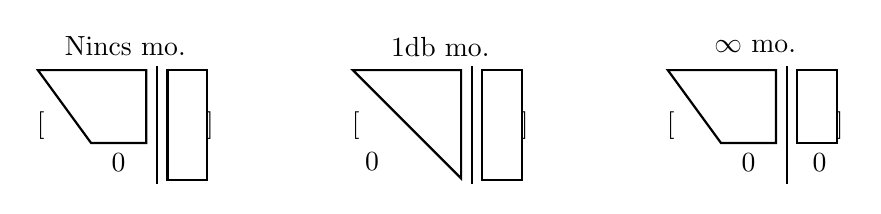
\begin{tikzpicture}[thick]
      \foreach \i in {0,1,2} {
          \node at (\i*4cm,0) {$\left[\phantom{\begin{matrix}10000000000\\\\\\\\\end{matrix}}\right]$};

          \draw (\i*4cm+4mm,.75cm) -- ++(0,-1.5cm);
        }

      \draw (5.35mm,7mm) rectangle ++(5mm, -14mm);
      \draw (45.35mm,7mm) rectangle ++(5mm, -14mm);
      \draw (85.35mm,7mm) rectangle ++(5mm, -9.25mm) node[below left] {$0$};

      \draw (2.65mm,7mm)
      -- ++(-13.75mm,0)
      -- ++(6.75mm,-9.25mm)
      -- ++(7mm,0)
      node[midway, below] {$0$}
      -- cycle;
      \draw (42.65mm,7mm)
      -- ++(-13.75mm,0)
      -- ++(13.75mm,-13.75mm)
      node[midway, below left=2.25mm] {$\quad0$}
      -- cycle;
      \draw (82.65mm,7mm)
      -- ++(-13.75mm,0)
      -- ++(6.75mm,-9.25mm)
      -- ++(7mm,0)
      node[midway, below] {$0$}
      -- cycle;

      \node[] at (0cm,1cm) {Nincs mo.};
      \node[] at (4cm,1cm) {1db mo.};
      \node[] at (8cm,1cm) {$\infty$ mo.};
    \end{tikzpicture}
  \end{block}
\end{frame}

\begin{frame}
  \frametitle{Lineáris egyenletrendszerek}
  \framesubtitle{Feladatok}

  \vfill
  \begin{exercise}{Oldjuk meg az alábbi lineáris egyenletrendszert!}
  \[
    \begin{array}{*{7}{c}}
      x_{1}   & + & 4 x_{2} & + & 8 x_{3} & = & 23 \\
              &   & x_{2}   &   &         & = & 1  \\
      2 x_{1} & + & 4 x_{2} & + & 6 x_{3} & = & 22
    \end{array}
  \]

  \exsol[14.25cm]{%
    Oldjuk meg a feladatot mátrix inverziós módszerrel! Írjuk fel az együttható
    mátrixot, az ismeretlenek vektorát és a konstans vektort:
    \[
      \rmat A = \begin{bmatrix}
        1 & 4 & 8 \\
        0 & 1 & 0 \\
        2 & 4 & 6
      \end{bmatrix}
      \text,
      \quad
      \rvec x = \begin{bmatrix}
        x_1 \\ x_2 \\ x_3
      \end{bmatrix}
      \text,
      \quad
      \rvec b = \begin{bmatrix}
        23 \\ 1 \\ 22
      \end{bmatrix}
      \text.
    \]

    Az $\rmat A$ mátrix inverzét már korábban meghatároztuk:
    \[
      \rmat A^{-1} = \begin{bmatrix}
        -3/5 & -4/5 & 4/5   \\
        0    & 1    & 0     \\
        1/5  & -2/5 & -1/10
      \end{bmatrix}
      \text.
    \]

    Az egyenletrendszer megoldása tehát:
    \[
      \rvec x
      = \rmat A^{-1} \rvec b
      = \begin{bmatrix}
        -3/5 & -4/5 & 4/5   \\
        0    & 1    & 0     \\
        1/5  & -2/5 & -1/10
      \end{bmatrix} \begin{bmatrix}
        23 \\ 1 \\ 22
      \end{bmatrix}
      = \begin{bmatrix}
        -3/5 \cdot 23 - 4/5 \cdot 1 + 4/5 \cdot 22 \\
        0 \cdot 23 + 1 \cdot 1 + 0 \cdot 22        \\
        1/5 \cdot 23 - 2/5 \cdot 1 - 1/10 \cdot 22
      \end{bmatrix}
      = \begin{bmatrix}
        3 \\ 1 \\ 2
      \end{bmatrix}
      \text.
    \]

    Tehát az egyes változók értékei: $x_1 = 3$, $x_2 = 1$, és $x_3 = 2$.

    \tcbline

    Oldjuk meg Gauss-eliminációval is az egyenletrendszert:
    \newcommand{\qgj}[6]{\left[\begin{array}{*{3}{X{8mm}}|X{8mm}}
          #1 \\#3\\#5
        \end{array}\right]\begin{matrix}#2\\#4\\#6\end{matrix}}
    \begin{align*}
         & \qgj
      {1 & 4    & 8   & 23}{}
      {0 & 1    & 0   & 1 }{}
      {2 & 4    & 6   & 22}{(-2S_1)}
      \\
         & \qgj
      {1 & 4    & 8   & 23 }{(-4S_2)}
      {0 & 1    & 0   & 1  }{}
      {0 & -4   & -10 & -24}{(+4S_2)}
      \\
         & \qgj
      {1 & 0    & 8   & 19 }{}
      {0 & 1    & 0   & 1  }{}
      {0 & 0    & -10 & -20}{(/(-10))}
      \\
         & \qgj
      {1 & 0    & 8   & 19}{(-8S_3)}
      {0 & 1    & 0   & 1 }{}
      {0 & 0    & 1   & 2 }{\;}
      \\
         & \qgj
      {1 & 0    & 0   & 3}{}
      {0 & 1    & 0   & 1}{}
      {0 & 0    & 1   & 2}{}
    \end{align*}
    % Látható, hogy ezzel a módszerrel is ugyan azokat a megoldásokat kaptuk.
  }
\end{exercise}

  \vfill
  \begin{exercise}{%
		Milyen együtthatók esetén nem lesz megoldható az egyenletrendszer
		Cramer-szabállyal?
	}
	\[
		\begin{array}{*{7}{c}}
			a x_{1}  & + & -2 x_{2} & + & 1 x_{3} & = & 1 \\
			-4 x_{1} & + & b x_{2}  & + & 2 x_{3} & = & 2 \\
			-8 x_{1} & + & 3b x_{2} & + & 4 x_{3} & = & 3
		\end{array}
	\]

	\exsol{%
		A Cramer-szabály akkor alkalmazható, ha az együttható mátrix reguláris.
		Írjuk fel a mátrixot, majd vizsgáljuk meg, hogy milyen együtthatók esetén
		lesz szinguláris, hiszen ilyen esetekben nem használható a Cramer-szabály:
		\[
			\rmat A = \begin{bmatrix}
				a  & -2 & 1 \\
				-4 & b  & 2 \\
				-8 & 3b & 4
			\end{bmatrix}
			\text.
		\]
		Az mátrix az alábbi esetekben lesz szinguláris:
		\begin{itemize}
			\item ha az első és a harmadik oszlop egymás skalárszorosa,
			      vagyis ha $a = -2$,
			\item ha a második és a harmadik sor egymás skalárszorosa,
			      vagyis ha $b = 0$.
		\end{itemize}
		Tehát a Cramer-szabályt akkor nem tudjuk alkalmazni,
		ha $a = 2$, ha vagy $b = 0$.
	}
\end{exercise}

  \vfill
\end{frame}
